
%%%%%%%%%%%%%%%%%%%%%%%%%%%%%%%%%%%%%%%%%%%%%%%%%%%%%%%%%%%%%%%%%%%%%
%% This is a (brief) model paper using the achemso class
%% The document class accepts keyval options, which should include
%% the target journal and optionally the manuscript type.
%%%%%%%%%%%%%%%%%%%%%%%%%%%%%%%%%%%%%%%%%%%%%%%%%%%%%%%%%%%%%%%%%%%%%
\documentclass[journal=apchd5,manuscript=article]{achemso}

%%%%%%%%%%%%%%%%%%%%%%%%%%%%%%%%%%%%%%%%%%%%%%%%%%%%%%%%%%%%%%%%%%%%%
%% Place any additional packages needed here.  Only include packages
%% which are essential, to avoid problems later. Do NOT use any
%% packages which require e-TeX (for example etoolbox): the e-TeX
%% extensions are not currently available on the ACS conversion
%% servers.
%%%%%%%%%%%%%%%%%%%%%%%%%%%%%%%%%%%%%%%%%%%%%%%%%%%%%%%%%%%%%%%%%%%%%
\usepackage[version=3]{mhchem} % Formula subscripts using \ce{}
\usepackage[T1]{fontenc}       % Use modern font encodings
\usepackage{graphicx}
\usepackage{amsmath}
\usepackage{xcolor}
\usepackage{wrapfig}
%\usepackage{multline}
%%%%%%%%%%%%%%%%%%%%%%%%%%%%%%%%%%%%%%%%%%%%%%%%%%%%%%%%%%%%%%%%%%%%%
%% If issues arise when submitting your manuscript, you may want to
%% un-comment the next line.  This provides information on the
%% version of every file you have used.
%%%%%%%%%%%%%%%%%%%%%%%%%%%%%%%%%%%%%%%%%%%%%%%%%%%%%%%%%%%%%%%%%%%%%
%%\listfiles

%%%%%%%%%%%%%%%%%%%%%%%%%%%%%%%%%%%%%%%%%%%%%%%%%%%%%%%%%%%%%%%%%%%%%
%% Place any additional macros here.  Please use \newcommand* where
%% possible, and avoid layout-changing macros (which are not used
%% when typesetting).
%%%%%%%%%%%%%%%%%%%%%%%%%%%%%%%%%%%%%%%%%%%%%%%%%%%%%%%%%%%%%%%%%%%%%
\newcommand*\mycommand[1]{\texttt{\emph{#1}}}

%%%%%%%%%%%%%%%%%%%%%%%%%%%%%%%%%%%%%%%%%%%%%%%%%%%%%%%%%%%%%%%%%%%%%
%% Meta-data block
%% ---------------
%% Each author should be given as a separate \author command.
%%
%% Corresponding authors should have an e-mail given after the author
%% name as an \email command. Phone and fax numbers can be given
%% using \phone and \fax, respectively; this information is optional.
%%
%% The affiliation of authors is given after the authors; each
%% \affiliation command applies to all preceding authors not already
%% assigned an affiliation.
%%
%% The affiliation takes an option argument for the short name.  This
%% will typically be something like "University of Somewhere".
%%
%% The \altaffiliation macro should be used for new address, etc.
%% On the other hand, \alsoaffiliation is used on a per author basis
%% when authors are associated with multiple institutions.
%%%%%%%%%%%%%%%%%%%%%%%%%%%%%%%%%%%%%%%%%%%%%%%%%%%%%%%%%%%%%%%%%%%%%
\author{Nicholas P. Montoni}
\author{Steven C. Quillin}
\author{Charles Cherqui}
\author{David J. Maisello}
\affiliation[Department of Chemistry, University of Washington]
{Department of Chemistry, University of Washington, Seattle, WA 98195}
\email{masiello@chem.washington.edu}
\date{February 12, 2017}
%%%%%%%%%%%%%%%%%%%%%%%%%%%%%%%%%%%%%%%%%%%%%%%%%%%%%%%%%%%%%%%%%%%%%
%% The document title should be given as usual. Some journals require
%% a running title from the author: this should be supplied as an
%% optional argument to \title.
%%%%%%%%%%%%%%%%%%%%%%%%%%%%%%%%%%%%%%%%%%%%%%%%%%%%%%%%%%%%%%%%%%%%%
\title[]
    {Tunable Spectral Ordering of Magnetic Plasmon Resonances}
%%%%%%%%%%%%%%%%%%%%%%%%%%%%%%%%%%%%%%%%%%%%%%%%%%%%%%%%%%%%%%%%%%%%%
%% Some journals require a list of abbreviations or keywords to be
%% supplied. These should be set up here, and will be printed after
%% the title and author information, if needed.
%%%%%%%%%%%%%%%%%%%%%%%%%%%%%%%%%%%%%%%%%%%%%%%%%%%%%%%%%%%%%%%%%%%%%
\abbreviations{MNP, LSPR, EELS}
\keywords{magnetic plasmons, plasmon metamolecules}

%%%%%%%%%%%%%%%%%%%%%%%%%%%%%%%%%%%%%%%%%%%%%%%%%%%%%%%%%%%%%%%%%%%%%
%% The manuscript does not need to include \maketitle, which is
%% executed automatically.
%%%%%%%%%%%%%%%%%%%%%%%%%%%%%%%%%%%%%%%%%%%%%%%%%%%%%%%%%%%%%%%%%%%%%
\begin{document}

%%%%%%%%%%%%%%%%%%%%%%%%%%%%%%%%%%%%%%%%%%%%%%%%%%%%%%%%%%%%%%%%%%%%%
%% The "tocentry" environment can be used to create an entry for the
%% graphical table of contents. It is given here as some journals
%% require that it is printed as part of the abstract page. It will
%% be automatically moved as appropriate.
%%%%%%%%%%%%%%%%%%%%%%%%%%%%%%%%%%%%%%%%%%%%%%%%%%%%%%%%%%%%%%%%%%%%%
\begin{tocentry}
\begin{centering}
\includegraphics[height=3.5cm]{toc.png}
\end{centering}
\end{tocentry}

%%%%%%%%%%%%%%%%%%%%%%%%%%%%%%%%%%%%%%%%%%%%%%%%%%%%%%%%%%%%%%%%%%%%%
%% The abstract environment will automatically gobble the contents
%% if an abstract is not used by the target journal.
%%%%%%%%%%%%%%%%%%%%%%%%%%%%%%%%%%%%%%%%%%%%%%%%%%%%%%%%%%%%%%%%%%%%%

\begin{abstract}
Abstract.
%Using first-principles theory and simulated cathodoluminescence spectroscopy, the optical-frequency magnetic resonances of cyclic aromatic and hexagonally packed metal nanoparticle clusters are explored. A fully retarded coupled dipole model is employed, expanding upon past work in the field, to explore the dependence of the resonant frequencies and spectral ordering of the magnetic resonances on cluster size. It is shown that magnetic resonances change spectral order as metal nanoparticle oligomers change in size, and that these mode switches are observable in full-wave numerical electrodynamics simulations of angle-resolved cathodoluminescence spectra. Electron-beam spectroscopies are uniquely suited to observing this phenomenon, as they provide nanometer spatial and sub-eV spectral resolution and can preferentially excite one magnetic resonance over another. Furthermore, angle-resolved spectroscopies leverage the specific radiation patterns attributed to each magnetic plasmon, clearly differentiating spectral signatures of each individual magnetic plasmon resonance.
\end{abstract}

%%%%%%%%%%%%%%%%%%%%%%%%%%%%%%%%%%%%%%%%%%%%%%%%%%%%%%%%%%%%%%%%%%%%%
%% Start the main part of the manuscript here.
%%%%%%%%%%%%%%%%%%%%%%%%%%%%%%%%%%%%%%%%%%%%%%%%%%%%%%%%%%%%%%%%%%%%%
Clusters of metal nanoparticles (MNPs) that exhibit anomalously strong magnetic fields, called plasmon oligomers or plasmon metamolecules, have been of great interest in recent years\cite{Alu2006,Alu2008,Liu2011,Dionne2011,Qian2015,Dionne2016}. Magnetic plasmon resonances in these systems have been shown to couple to and enhance the magnetic field of light and hybridize analogously to electric plasmon resonances\cite{Zhang2006,Zhang2007,NordHal2011,NordHal2012,Cherqui2014,Cherqui2016,Engheta2017}. The magnetic properties of single oligomers, i.e. those systems composed of only one ring of MNPs, are now well understood based upon models in the quasistatic limit\cite{Nord2006,Dionne2011,Dionne2016,Capolino2017}. Conversely, the infinite-oligomer regime has also been understood within the language of tight-binding models of solid-state physics\cite{Schatz2003,Weick2013}. Recently, a disconnect between these size regimes and methods has arisen, leading to open questions in how magnetic plasmon resonances behave in few-oligomer assemblies, called the intermediate size regime\cite{NordHal2011,NordHal2012,Cherqui2014,Cherqui2016,Engheta2017}.

Most crucial to this disconnect is the question of when and how retardation effects matter. For example, in the case of the two oligomer cluster (the 2-mer) the quasistatic approximation has been shown to deviate from full-wave numerical electrodynamics simulations in that it predicts a different energy-ordering of the magnetic plasmon resonances.\cite{Cherqui2014} Retardation effects have been incorporated into models of single MNPs\cite{Gu2010}, dimers\cite{Oubre2004,vonPlessen2007}, and infinite chains and arrays\cite{Lucas1976,ARAVIND1981,Kottman2001,NordHal2003,NordProdan2004,Rechbacher2003,Schatz2003,Royer2005,Abajo2008,Gomez2009,Chumanov2010,Pinchuk2016}. However, with the exception of numerical studies, no analytical models include retardation effects in the description of magnetic plasmon oligomers. Here, we show that the incorporation of retardation effects corrects the aforementioned discrepancy between model and simulation, and further points to the facile ability to tune the magnetic plasmon spectrum via scaling oligomer size. This is important because it allows for the facile manipulation of the effective permittivity and permeability thereby facilitating the design of future tunable optical metamaterials.

In the following, we demonstrate the evolution of the magnetic plasmon resonances in intermediate-size $N$-mers with size by including the full field within a coupled dipole approach describing their interaction. Interestingly, as a function of size, the magnetic resonances switch their ordering in analogy to the way that electric plasmon resonances in hybridized nanoparticles can switch order\cite{vonPlessen2007}. We further analyze the distinct radiative properties of each magnetic plasmon resonance by computing the angle-resolved cathodoluminescence (CL) spectrum\cite{Hohenester2014,Coenen2011,CoPol2011,Polman2014}. The spectral ordering depends not only on aggregate size but also upon oligomer morphology which we examine below. The ability to choose the resonance frequency of specific magnetic plasmon resonances will lead to advances in superlensing and electromagnetic cloaking at optical frequencies, as these applications stem directly from tunable negative-index metamaterials\cite{Pendry03,Fang2005,Cai2007,Pinchuk07,Shalaev2008,Valentine2008,Ferrari09}.

\section{Model Theory}

\begin{figure}
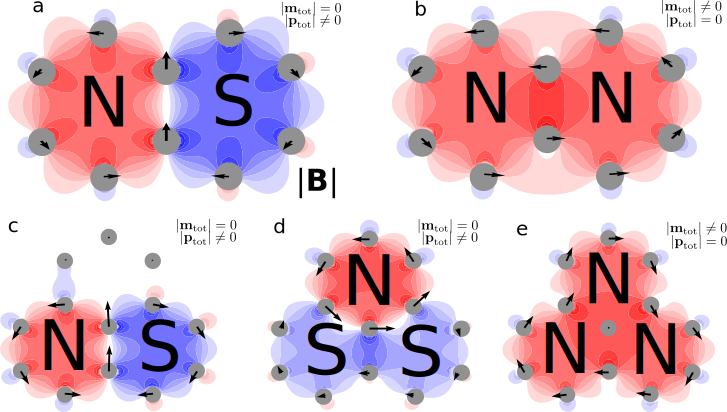
\includegraphics{2mer_3mer_fields.pdf}
\caption{Magnetic field plots of the 2mer (a and b) and 3mer (c, d, and e) oligomers. Each system supports a number of closed-loop magnetic plasmon resonances equal to the number of rings in the system. The magnetic plasmons support an electric dipole moment (a, c, and d) support out-of-phase magnetic fields. The nodeless magnetic modes (b and e) support a net magnetic dipole moment are accessible to the magnetic field of light.}
\label{field_plots}
\end{figure}

Figure~\ref{field_plots} displays two model systems, the 2-mer and 3-mer, comprising 10 and 13 silver nanospheres in analogy to naphthalene and phenalene. The mapping of the electric localized surface plasmon resonances of individual noble metal nanoparticles onto harmonic oscillators is now well-understood\cite{ARPC}. In the limit where each nanoparticle, here restricted to a spherical geometry of radius $a$, possesses only an electric dipole plasmon resonance, the equations of motion dictating the electromagnetic response of the oligomer are

\begin{equation}
\ddot{\textbf{q}}_i = -\omega_{\textrm{sp}}^2\textbf{q}_i + \frac{e}{m_{\textrm{sp}}}\sum_{i,j\neq i}\textbf{E}_j(\textbf{r}_i),
\label{equation_of_motion}
\end{equation}

\noindent where $\omega_{\textrm{sp}}$ is the natural frequency of the Mie resonance, $m_{\textrm{sp}} = e^2/\alpha_{\textrm{sp}}\omega_{\textrm{sp}}^2$ is the plasmon's effective mass defined in terms of the polarizability $\alpha_{\textrm{sp}} = 3a^3/(\varepsilon_{\infty} + 2\varepsilon_b)$, with $\varepsilon_{\infty}$ and $\varepsilon_b$ the high-frequency and background dielectric functions. The dipole moment of each plasmon oscillator, restricted to lie in the plane of the oligomer at position $\textbf{r}_i$, is $\textbf{d}_i = e\textbf{q}_i$ and $\textbf{E}_j(\textbf{r}_i)$ is the fully retarded electric field of the $j^{\textrm{th}}$ dipole evaluated at the position of the $i^{\textrm{th}}$ dipole. The electric field is defined by

\begin{equation}
\textbf{E}_j(\textbf{r}_i) = \boldsymbol{\Lambda}_{ij}\cdot\textbf{d}_j\\
= \left\{\left(\frac{1}{r_{ij}^3} - \frac{ik}{r_{ij}^2}\right)\left(3\hat{\textbf{n}}_{ij}\hat{\textbf{n}}_{ij} - \textbf{1}\right) - \frac{k^2}{r_{ij}}\left(\hat{\textbf{n}}_{ij}\hat{\textbf{n}}_{ij} - \textbf{1}\right)\right\}\frac{e^{\textrm{i}kr_{ij}}}{\varepsilon_b}\cdot\textbf{d}_j,
\label{electric_field_lambda}
\end{equation}

\noindent where, $\hat{\textbf{n}}_{ij}$ is the unit vector connecting two dipoles separated by distance $r_{ij}$, $k=\sqrt{\varepsilon_b}\omega/c$ where $\omega$ is the oscillatory frequency of the $j^{\textrm{th}}$ dipole. Interestingly, the far-field term carries the opposite sign of the near-field term. The field is decomposed into three parts: the near- ($r_{ij}^{-3}$), intermediate- ($r_{ij}^{-2}$), and far-field ($r_{ij}^{-1}$). All dipolar retardation effects are included in this field\cite{Purcell1973}. Due to the relative magnitudes of these terms and the sign of $e^{\textrm{i}kr_{ij}}$ the interaction energies can change sign and go from energy-lowering to energy-raising.

As described in the methods section, there are as many normal modes of each N-mer as there are electric dipole plasmons. Of these normal modes, some are electric in character and some are magnetic in character with $N$ magnetic plasmon resonances for each $N$-mer studied here. Figure~\ref{field_plots} shows these magnetic plasmon normal modes overlaid with their associated signed magnetic field magnitude. Each mode is named for its particular magnetic field distribution after the poles of a magnet, either all-North (aN) or North-South (NS). The top right-hand corner of each panel indicates whether the  mode depicted has a net electric dipole or a net magnetic dipole moment. In planar geometries, the magnetic dipole moments are always perpendicular to the in-plane electric dipole moments. As a result, they scatter light with different directionality as will be discussed.

\section{Spectral Ordering of Magnetic Modes in Model Systems}

To determine the impact of incorporating retardation effects, it is first useful to consider the quasistatic limit. Here individual particle frequencies (define omegasp) are size independent and the coupling strength depends only upon the scale $s = r_{ij}/a$ and not upon the overall oligomer size. That is, if this ratio $s$ of inter-particle distance $r_{ij}$ to particle size $a$ remains constant, as the particles grow the collective frequencies do not change. This is evident by considering the k goes to zero limit of the electric field in Equation~\ref{electric_field_lambda},

\begin{equation}
\begin{aligned}
\lim_{k \to 0}\textbf{E}_j(\textbf{r}_i) &= \frac{e^2}{m_{\textrm{sp}}}\boldsymbol{\Lambda}_{ij}\\ 
&= \frac{\omega_{\textrm{sp}}^2 \alpha_{\textrm{sp}}^2}{\varepsilon_b}\frac{3\hat{\textbf{n}}_{ij}\hat{\textbf{n}}_{ij} - \textbf{1}}{r_{ij}^3} \cdot \textbf{d}_j \\
&= \frac{\omega_{\textrm{sp}}^2}{\varepsilon_b} \left(\frac{3}{\varepsilon_{\infty}+2\varepsilon_b}\right)\frac{3\hat{\textbf{n}}_{ij}\hat{\textbf{n}}_{ij} - \textbf{1}}{s^3} \cdot \textbf{d}_j
\end{aligned}
\label{quasistatic_coupling}
\end{equation}

\noindent where $m_{\textrm{sp}}$ and $\alpha_{\textrm{sp}}$ are rewritten in terms of fundamental parameters for silver: $\varepsilon_{\infty} = 3.77$, $\hbar\gamma = 0.05$ eV, and $\hbar\omega_{p} = 9.1$ eV. Retardation effects, however, remove this invariance and introduce size-dependence into both the individual plasmon natural frequency as well as into the electric field. Consequently, in the following we choose the individual MNP radius $a$ as the independent variable, fixing the nearest neighbor distance at 3$a$, to investigate the effects of retardation upon the magnetic plasmon spectrum in intermediate-size $N$-mers.

\begin{figure}
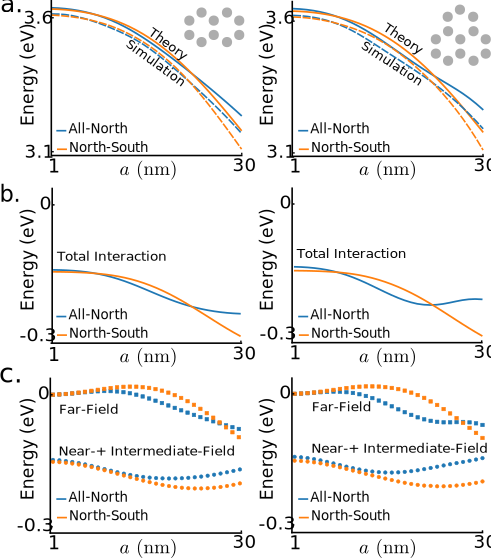
\includegraphics{2mer-3mer-eig.pdf}
\caption{Eigenenergies (a and c) and interaction energies (b and d) for the 2mer and 3mer. At small scales $r_0 < 5$ nm the magnetic modes are ordered as predicted using a quasistatic model, with NS (orange) lower in energy than aN (blue). This implies that for very small oligomer systems, the quasistatic approximation is still accurate. However, at sizes greater than $r_0 = 5$ nm and smaller than $r_0 = 20$ nm, the eigenmodes switch order. This is due to the dominance of the far-field term, which is evident from (b and d). Finally, at sizes greater than $r_0 = 20$ nm, the eigenmodes switch order again. Also plotted are simulated peak positions of each mode (dashed lines) to show agreement within 0.1 eV.}
\label{scaling}
\end{figure}

Figure~\ref{scaling} shows the predicted resonance energies from both the model and full-wave optical simulations of the 2-mer and 3-mer with increasing $a$.\cite{Hohenester2012} At small sizes the magnetic modes preserve the quasistatic ordering predicted in previous work, which is to be expected when the oligomer system fits within a wavelength of light and the near-field dominates the electric field\cite{Cherqui2014}. As the system size increases, the resonance energies decrease and to cross at $a = 7$ nm, and once more at $a = 20$ nm. This is due to the far-field contribution in Equation~\ref{electric_field_lambda} becoming large relative to the near- and intermediate-fields, as shown in Figure~\ref{scaling}b and d (squares). The second crossing of the eigenmodes recovers the ordering at small sizes, which might lead to the erroneous conclusion that the quasistatic approximation is accurate again. Rather, both eigenmode crossings are due entirely to retardation effects. The interaction energy between all the dipoles in each magnetic mode, [reformat equation]

\begin{equation}
U_{\textrm{int}} = -\frac{1}{2} \sum_{ij} \textbf{d}_i \cdot \textbf{E}_j(\textbf{r}_i),
\label{interactionenergy}
\end{equation}

\noindent with the same $\textbf{E}_j$ defined in Equation~\ref{electric_field_lambda}, explains why the modes cross at certain system sizes. The inclusion of the far-field, the third term in Equation~\ref{electric_field_lambda} is the cause of the mode switching, as it carries the opposite sign of the near- and intermediate-field terms. These terms with opposite splitting are the cause of the mode crossings; as the near- and intermediate-fields lower the energy of the North-South mode, the far-field raises the energy of the North-South mode, and vice-versa for the North-North mode. Close inspection of Figure~\ref{scaling}b reveals that the crossing points occur where the splitting in the near- and intermediate-fields is equal and opposite to that of the far-field. Perhaps more interestingly, in any dielectric medium with $\varepsilon_b > 1$ the crossing points are shifted towards smaller scale due to wavelength contraction. This can also be explained through the impact of a dielectric medium on coupling strength. While a medium should contribute an overall increase to the coupling strength, the far-field term should be more drastically impacted due to its extra $\varepsilon_b$-dependence through its $k^2$ term.\cite{Elsayed2008}

Previous work has explored the oscillatory nature of hybridized electric dipole plasmon resonance frequencies and radiation damping as a function of separation in noble metal dimers\cite{vonPlessen2007}. Analogously, our work shows that magnetic plasmon resonance energies also oscillate with interparticle separation and can be understood via analysis of the contributions to the dipole-dipole interaction.

\section{Radiative Properties of Magnetic Plasmon Resonances}
Only those magnetic resonances supporting net electric or magnetic dipole moments will radiate to the far field. The magnetic dipole moment of the aN magnetic mode is perpendicular to the electric dipole moment(s) of the NS mode in both the model 2-mer and 3-mer. This means that these modes radiate with different directionality. It has been predicted and shown experimentally that 1-mers scatter light anisotropically when both their magnetic dipole moment and electric dipole moment are mutually excited,\cite{Dionne2011,Cherqui2016} as is evident in differential scattering spectra and profiles. Both observations stem from the differential power,\cite{jackson_classical_1999,schwinger1998classical}

\begin{equation}
\frac{dP}{d\Omega} = \frac{c}{8\pi}\textrm{Re}\left[r^2\hat{\textbf{n}}\cdot\sum_i\textbf{E}_i \times \sum_{j}\textbf{B}_{j}^*\right]
\label{dp_field_1}
\end{equation}

\noindent $\textbf{E}_i$ and $\textbf{B}_i$ are produced from the sum of effective electric ($\textbf{d}_i$) and magnetic ($\boldsymbol{\mu}_i$) dipole moments of each ring of the $N$-mer, assumed to be co-located at the center of the $i$-th ring and oscilalting in time as $e^{-\textrm{i}\omega t}$. In this approxiamtion, the differential power becomes\cite{Alu2006}

\begin{equation}
\begin{aligned}
\frac{dP}{d\Omega} &= \frac{ck^4}{8\pi} \textrm{Re} \left\{\hat{\textbf{n}} \cdot \left[\left(\sum_{i} (\hat{\textbf{n}} \times \textbf{d}_i) \times \hat{\textbf{n}} - \hat{\textbf{n}} \times \boldsymbol{\mu}_i\right) \times \left(\sum_{j} \hat{\textbf{n}} \times \textbf{d}_j^* + (\hat{\textbf{n}} \times \boldsymbol{\mu}_j^*) \times \hat{\textbf{n}}\right)\right]\right\}\\
&= \frac{ck^4}{8\pi} \textrm{Re} \Bigg[ \sum_{ij} \textbf{d}_i \cdot \textbf{d}_j^* - (\hat{\textbf{n}} \cdot \textbf{d}_i)(\hat{\textbf{n}} \cdot \textbf{d}_j^*) + \boldsymbol{\mu}_i \cdot \boldsymbol{\mu}_j^* - (\hat{\textbf{n}} \cdot \boldsymbol{\mu}_i)(\hat{\textbf{n}} \cdot \boldsymbol{\mu}_j^*) \\ &+ \hat{\textbf{n}} \cdot (\textbf{d}_i \times \boldsymbol{\mu}_j^* + \textbf{d}_j^* \times \boldsymbol{\mu}_i) \Bigg].
\label{dp_dipoles_1}
\end{aligned}
\end{equation}

\noindent Notice that the first two terms are due to electric and magnetic dipole radiation, while the third term is due to their interference. To build intuition, we demand the magnetic dipole $\boldsymbol{\mu}$ is oriented in the z-direction, and the electric dipole $\textbf{d}$ is oriented in the y-direction. The coarse-grained electric dipole and magnetic dipole can be written in terms of their constituent dipoles $\textbf{d} = \sum_n d_{e,n} \hat{\textbf{y}}$ and $\boldsymbol{\mu} = \frac{k}{2}\sum_n(\textbf{r}_n \times d_{m,n} \hat{\boldsymbol{\phi}}_n) = \frac{kNRd_m}{2}\hat{\textbf{z}}$ where the sums are taken over the $n$-th and $m$-th dipoles, respectively.

\begin{figure}
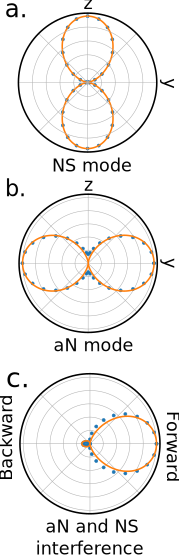
\includegraphics{differential_power_diagrams.pdf}
\caption{Magnetic field distributions of a magnetic dipole mode (a) and an electric dipole mode (c) in the xy-plane with corresponding radiation patterns (b and d) in the yz-plane. The magnetic dipole exhibits the expected dipolar doughnut, or two lobe, shape with a node along the z-axis. The electric dipole moment also shows the expected pattern with a node along the y-axis.}
\label{scattering}
\end{figure}

Figure~\ref{scattering} displays the differential power profiles associated with the aN and NS magnetic plasmon resonances, as well as the interference pattern, of any $N$-mer. Since the aN mode has only a z-oriented magnetic dipole, its radiation pattern is orthogonally oriented with respect to that of the y-directed electric dipole of the NS mode. Thus, examination of the directionality of radiation allows one to determine the net electric or magnetic dipole character. Strong forward/backward scattering asymmetries are also predicted and demonstrated in metal-semiconductor core-shell nanoparticle assemblies, which similarly exploit the interference between electric and magnetic plasmons\cite{Kivshar2012}.

\section{Angle-Resolved Cathodoluminescence for Observing Spectral Switching}
Recent studies have demonstrated the utility of angle-resolved CL spectroscopy to characterize plasmon resonances in noble metal nanoparticles\cite{Coenen2011,CoPol2011,Abajo2013,Polman2014,ARPC}. Using an electron microscope fitted with a parabolic mirror, emitted CL radiation can be collected across a large portion of the backward scattering hemisphere\cite{Coenen2011,CoPol2011,Polman2014}. Here we show that with the selection rules imposed by the location of the electron beam and the specific directionality of the emission from each magnetic mode, the magnetic modes of the $N$-mers and their crossings can be observed in angle-resolved CL spectra. The previous section built up intuition regarding the directionality of light scattered by the magnetic modes of the 2-mer and 3-mer. This intuition informs the particular angles at which to collect CL spectra associated with each magnetic mode. More specifically, based upon the selection rules imposed by the electron beam and the directionality of CL radiation, it is possible to distinguish the magnetic modes and their spectral ordering as a function of size.

\begin{figure}
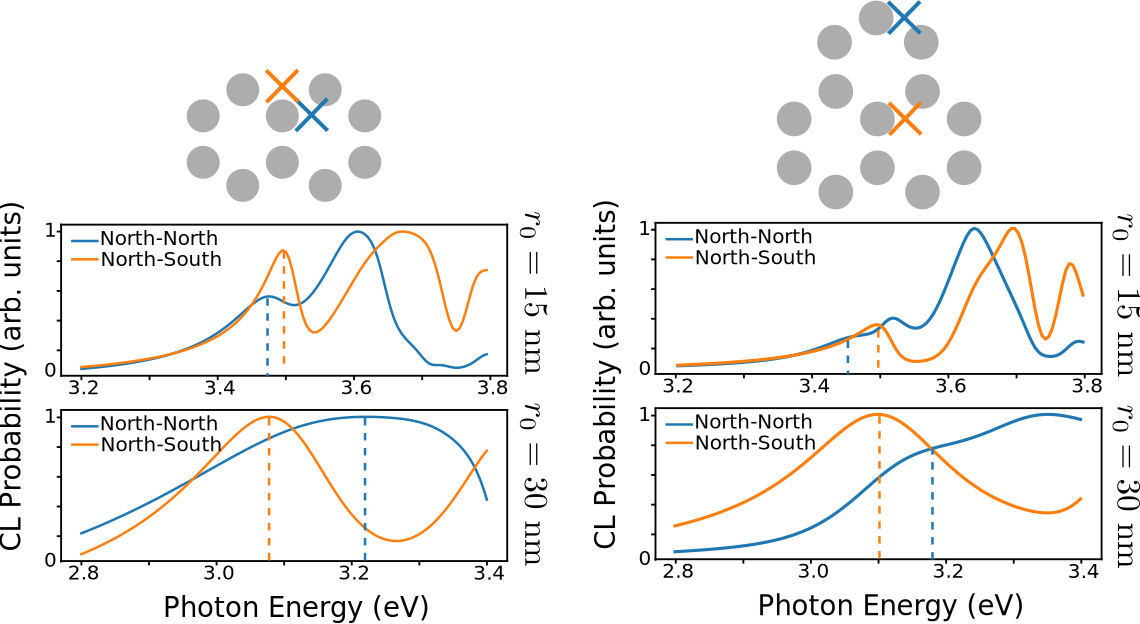
\includegraphics{CL_incomplete.pdf}
\caption{Angle-resolved cathodoluminescence spectra of the 2mer (a and b) and 3mer (c and d). By choosing the beam positions marked on the diagrams and choosing different angles at which to measure the light emitted, the magnetic modes of each oligomer can be disentangled. The colored "x's" correspond to colored traces. The blue traces show a collection angle of $\phi = 3\pi/2$ and the orange traces are for $\phi = \pi$, while both have $\theta = \pi/4$. Simulating these CL experiments with $r_0 = 15$ nm shows the aN modes lower in energy than the NS modes, as predicted. With $r_0 = 30$ nm, the modes switch, again as predicted.}
\label{CL_2mer_3mer}
\end{figure}

In Figure~\ref{CL_2mer_3mer} we show simulated point angle-resolved CL spectra of the 2-mer and 3-mer, with the electron beam position chosen so as to excite the aN (blue) and NS (orange) modes. Note however, due to the symmetry of the oligomers, the blue electron beam position excites not only the aN mode, but also weakly the NS mode. Since the radiation profile of the aN mode is orthogonal to that of the NS mode, it is possible to distinguish them by analyzing the angular distribution of emitted CL radiation. The ARCL spectra at two such angles are reported in Figure~\ref{CL_2mer_3mer}. These simulated spectra confirm the predictions of our model shown in Figure~\ref{scaling}; specifically, between $a = 15 - 30$ nm, the aN and NS modes switch spectral order.

\section{Magnetic Plasmon Resonance Frequencies and CL Spectra of Hexagonally-Packed Nanoclusters}

Ref. \cite{Engheta2017} synthesizes and optically characterizes hexagonally-packed nanoclusters composed of noble metal nanoparticles in the intermediate size regime, between few particle oligomers and infinite arrays. Here, we apply our analytical modeling and numerical simulation to investigate the behavior of the magnetic plasmon resonances as a function of size, with an eye toward engineering magnetic resonances at particular resonance energies. Such tunability may be important in the design of future negative index materials with spectral tunability. Specifically, we consider hexagonally packed clusters composed of 13, 19, and 31 MNPs displayed in Figure~\ref{kagan_fields} as well as the insets of Figure~\ref{kagan_eigen}.

\begin{figure}
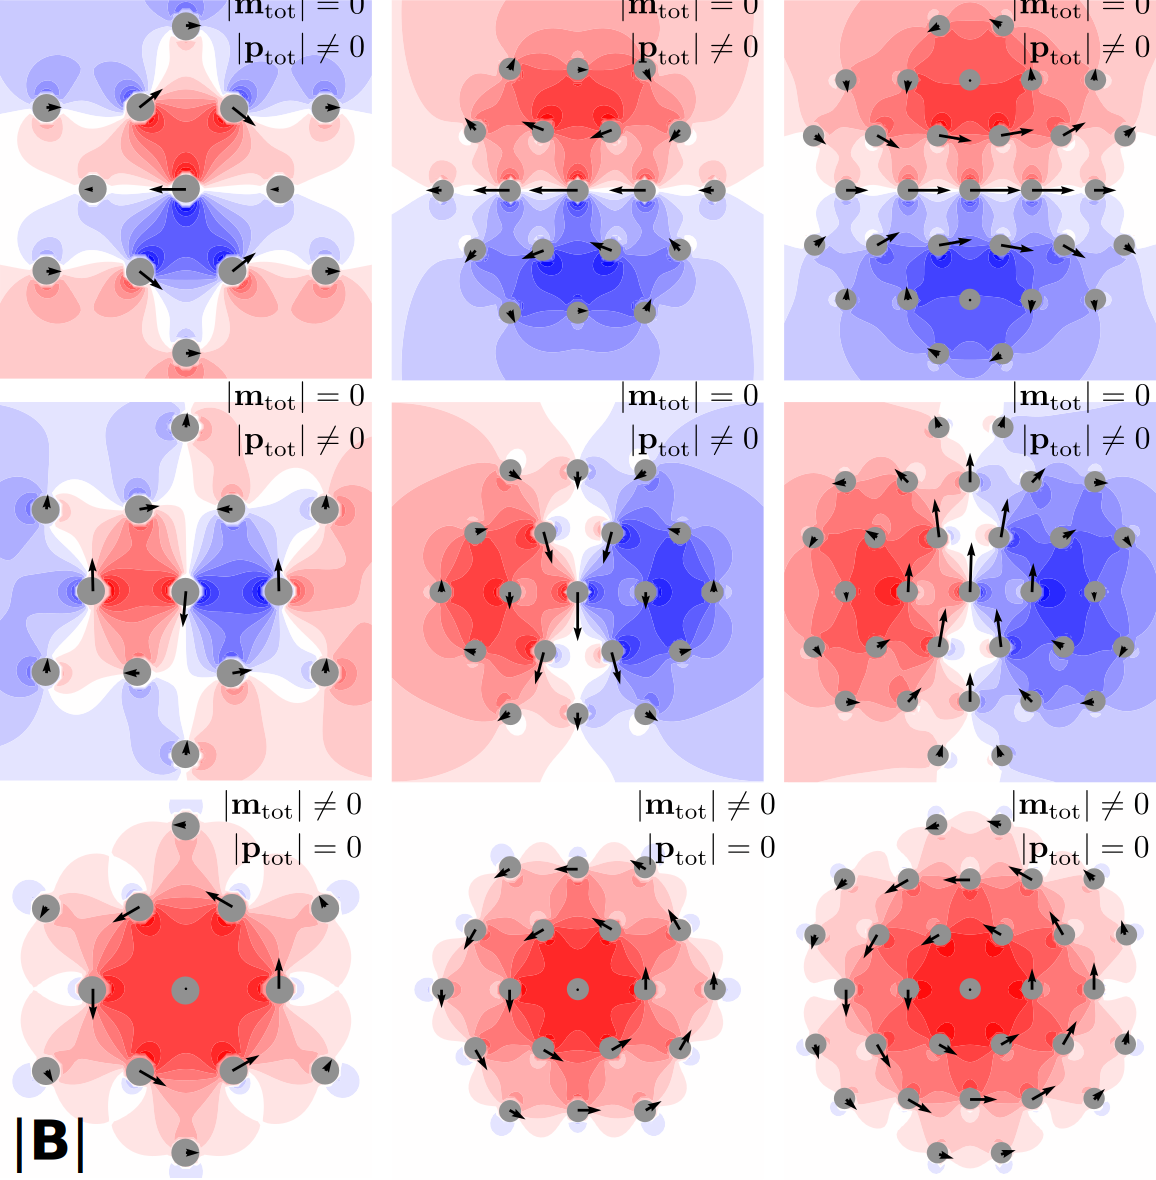
\includegraphics{kagan_fields.pdf}
\caption{Signed magnetic field magnitudes of the modes of the 13-particle (a, b, and c), 19-particle (d, e, and f), and 31-particle (g, h, and i) clusters. Similarly to the 2mer and 3mer from before, we present only those magnetic modes with either NS and electric dipole character (a, b, d, e, g, and h) or with aN and magnetic dipole character (c, f, and i).}
\label{kagan_fields}
\end{figure}

Figure~\ref{kagan_fields} displays the signed magnetic field magnitude of two magnetic plasmon resonances of the 13-, 19-, and 31-particle hexagonally packed nanoclusters. The NS mode of each nanocluster is doubly degenerate as would be true of any structure with sixfold symmetry. In analogy to the previous oligomers, these magnetic modes are chosen because they are spectrally isolated from the other magnetic modes and because their radiation patterns are spatially orthogonal. The arrows denote the electric dipole moments on individual nanoparticles within the magnetic normal mode and the color denotes the strength of the magnetic field. The net electric or magnetic dipole character of each magnetic resonance is denoted in the upper right hand corner of each panel.

Figure~\ref{kagan_eigen} displays the evolution of the aN and NS magnetic resonances with size, $a$. In contrast to the oligomers described previously, here the behavior of the nanocluster resonances with size is different due to the hexagonal packing as opposed to the open-ring structure of the oligomers. Nevertheless, the analytic model described previously is capable of predicting the magnetic spectrum. Most surprising is the behavior of the magnetic resonances of the 19- and 31-particle nanoclusters to oscillate with size as opposed to monotonically decrease in energy. Panels b, d, and f of Figure~\ref{kagan_eigen} display the relative strength of the near, intermediate, and far-field contributions to the electric dipole-electric dipole interaction energy and show that this oscillatory behavior is due specifically to retardation effects. This is contrary to intuition where increasing size causes monotonic redshifting. However this oscillatory behavior is not so unexpected; separating a MNP dimer causes its hybridized electric plasmon resonance frequencies to oscillate from bonding to anti-bonding and back\cite{vonPlessen2007}. In these nanoclusters, ARCL and patterns spectra provide a means to demonstrate this oscillation.

\begin{figure}
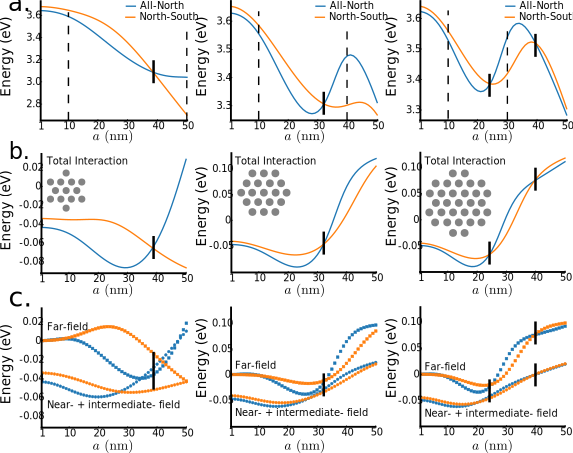
\includegraphics{13_19_31_eigen.pdf}
\caption{Eigenenergies and interaction energies for the magnetic modes of the 13- (a and b), 19- (c and d), and 31-particle (e and f) clusters. Unlike the previous 2mer and 3mer, at very small values of $r_0$, the aN modes are lower in energy than the NS modes. However, for each system a crossing point does occur between $r_0 = 30$ nm and $r_0 = 40$ nm. While the modes of the 13-particle system behave as expected, the aN and NS modes of the larger clusters behave contrary to the intuition built from the earlier model systems. At larger sizes, instead of a monotonic decrease in eigenenergies, the modes exhibit an increase in energy. Looking at the interaction energies, it becomes clear that this is again due to retardation effects, as the term that contributes the most anti-bonding character to the total interaction energy is the far-field. Furthermore, the 31-particle system exhibits a second crossing, unlike the other two structures, and the increase in its eigenenergies is maximized at smaller sizes.}
\label{kagan_eigen}
\end{figure}

\begin{figure}
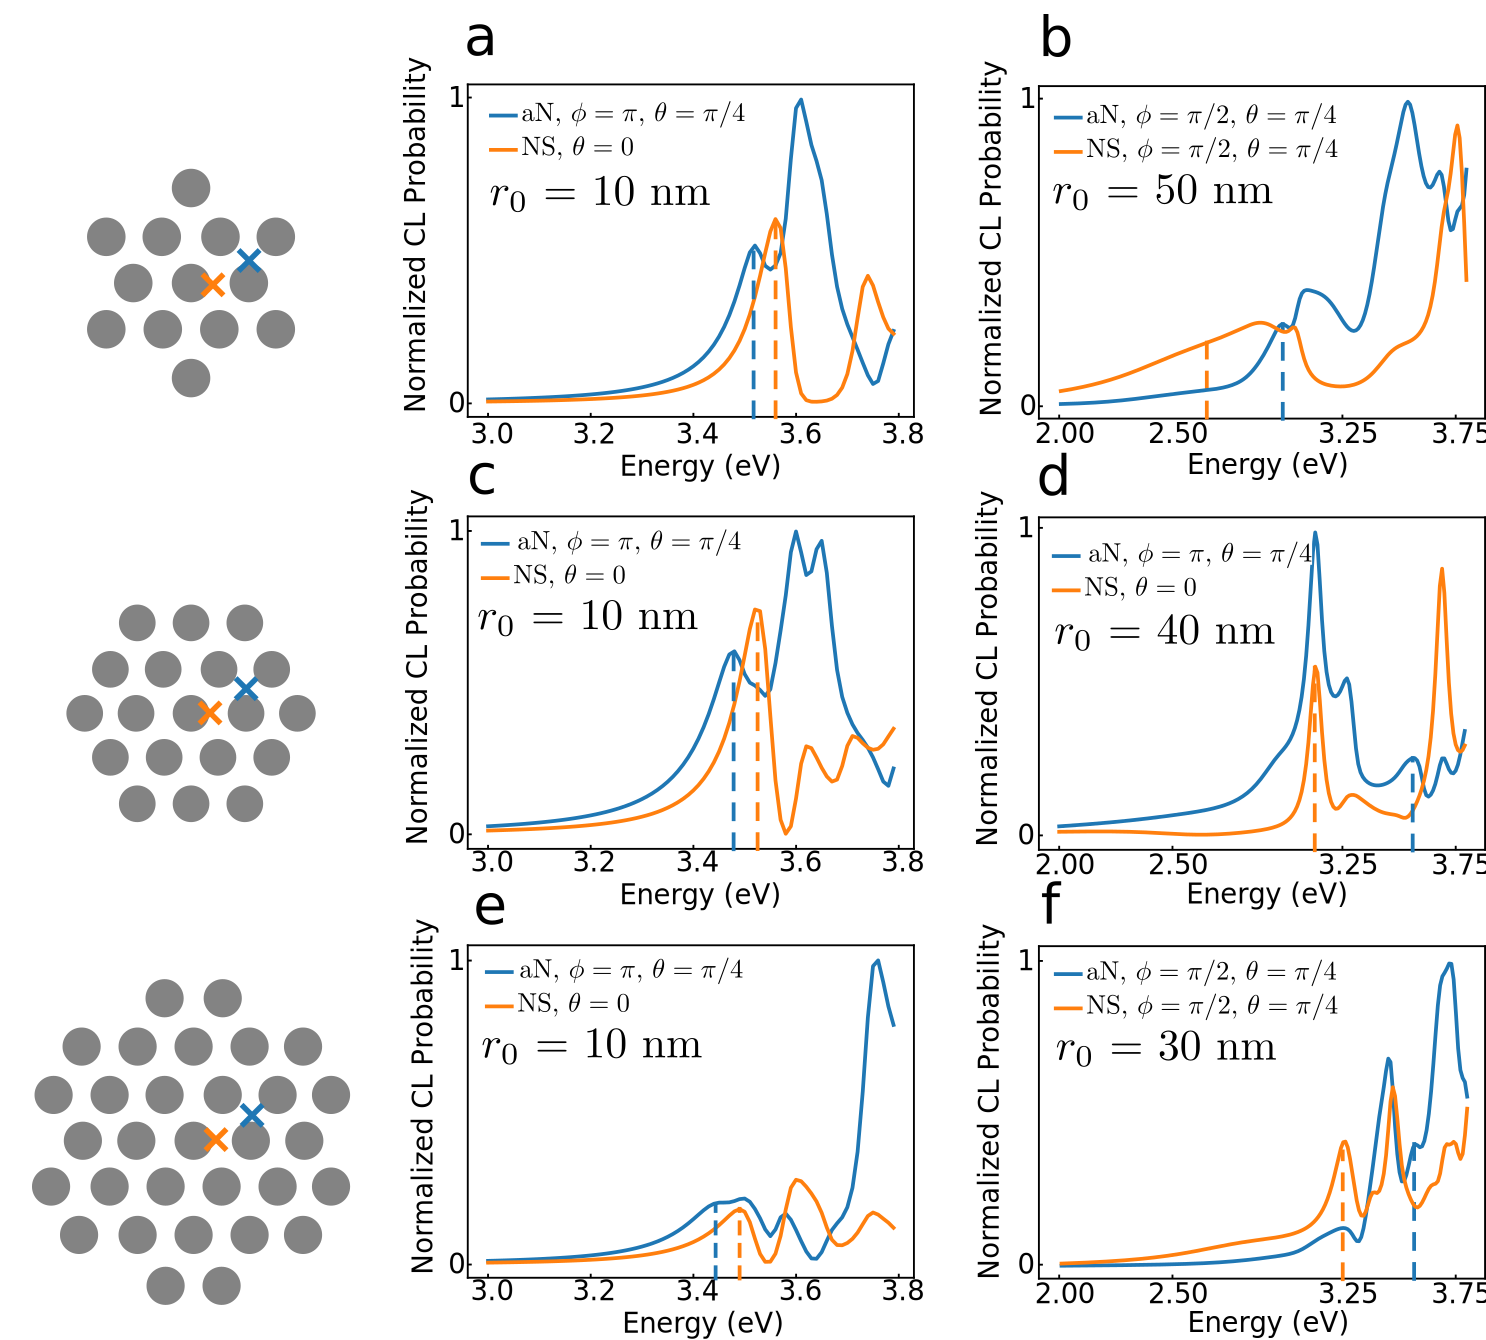
\includegraphics{kagan_CL_spectra.pdf}
\caption{Simulated angle-resolved cathodoluminescence spectra of the 13-, 19-, and 31-particle systems. Blue spectra were acquired at the beam positions marked with a blue x in order to preferentially excite the aN mode. Orange spectra were collected at the points marked with an orange x in order to preferentially excite the x-polarized NS mode. Spectra for the 13-particle aggregate were computed for $r_0 = 10$ nm (a) and $r_0 = 50$ nm (b). Spectra for the 19-particle aggregate were computed for $r_0 = 10$ nm (c) and $r_0 = 40$ nm (d). Spectra for the 31-particle aggregate were computed for $r_0 = 10$ nm (e) and $r_0 = 30$ nm (f). The dashed lines in each spectrum indicate the peak location of the aN modes (blue curves) and the NS modes (orange curves). Each panel also displays the collection angles for each spectrum.}
\label{kagan_CL}
\end{figure}

Figure~\ref{kagan_CL} shows simulated ARCL spectra for the 13-, 19-, and 31-particle systems acquired at the two indicated beam positions and collection angles. Inspection of the EELS maps of the NS and aN magnetic resonances in rows b and d of Figure~\ref{kagan_fields} indicates the optimal electron beam positions, that is, those positions with highest EEL probability, at which to excite each magnetic mode. As described previously, it is the electron beam selection rules and radiative profile of each mode help to identify the two magnetic resonances of interest. Because the aN mode radiates strongly in the xy-plane, and weakly in the z-direction, it is most easily detected at angles of $0 < \theta < \pi/2$. The NS mode is detected either for angles very close to the backward scattering direction ($\theta \approx 0$), or parallel to the impact plane (here, the y-direction for this particular beam position). The aN beam position also weakly excites the degenerate NS modes, meaning the corresponding CL spectrum will provide a secondary signature of the spectral location of that mode.

\section{Conclusion}
This paper is concluded.

\section{Methods}
Here we show how to derive the equations of motion describing magnetic plasmon resonances in nanoparticle clusters. References 10 and 43 describe how to map the solutions of Maxwell's Equations for electric plasmon resonances onto mechanical oscillators with effective masses. The resulting Hamiltonian for a system of $N$ frictionless coupled oscillators is

\begin{equation}
H = \sum_{i}\frac{\textbf{p}_i^2}{2m_{\textrm{sp}}}+\frac{1}{2}m_{\textrm{sp}}\omega_{\textrm{sp}}^2\textbf{q}_i^2 - \frac{e}{2}\sum_{ij,i\neq j}\textbf{q}_i\cdot\textbf{E}_j(\textbf{r}_i),
\label{hammy}
\end{equation}

\noindent where qi and $\textbf{p}_i$ are the coordinate and momentum of each plasmon oscillator located at $r_i$ with effective mass $m_{\textrm{sp}}$ and resonance frequency $\omega_{\textrm{sp}}$, defined previosuly; $\textbf{E}_j(\textbf{r}_i)$ is the full electric dipole field presented in Equation~\ref{electric_field_lambda}. The resulting equations of motion are,

\begin{equation}
\ddot{\textbf{q}}_i = -\omega_{\textrm{sp}}^2\textbf{q}_i + \frac{e}{m_{\textrm{sp}}}\sum_{j\neq i}\textbf{E}_j(\textbf{r}_i,\omega)
\label{equation_of_motion_again}
\end{equation}

\noindent which is exactly Equation~\ref{equation_of_motion}. From here, introducing time-dependence as a complex exponential, rewriting the electric field in terms of the plasmon coordinate, and performing a Fourier transform results in equations of motion in the frequency domain

\begin{equation}
(\omega_{\textrm{sp}}^2-\omega^2)\textbf{q}_i -\frac{e^2}{m_\textrm{sp}}\sum_{j\neq i}\boldsymbol{\Lambda}_{ij}(\omega)\cdot\textbf{q}_j = 0.
\label{fourier_eom}
\end{equation}

It is this system of equations for the plasmon oscillator coordinates that we solve for the normal modes. Considering two identical, coupled, collinear oscillators as an example with dipole-dipole coupling strength $g_{12} = $ Equation 13 becomes

\begin{equation}
(\omega_{\textrm{sp}}^2-\omega^2)q_1 -g_{12}(\omega)q_2 = 0
\label{fourier_eom_1}
\end{equation}

and

\begin{equation}
(\omega_{\textrm{sp}}^2-\omega^2)q_2 -g_{12}(\omega)q_1 = 0,
\label{fourier_eom_2}
\end{equation}

or equivalently

\begin{equation}
\begin{bmatrix}
(\omega_{\textrm{sp}}^2-\omega^2) & -g_{12}(\omega)\\
-g_{12}(\omega) & (\omega_{\textrm{sp}}^2-\omega^2)
\end{bmatrix}
\begin{bmatrix}
q_1\\
q_2
\end{bmatrix}
=
\begin{bmatrix}
0\\
0
\end{bmatrix}
\label{eom_matrix}
\end{equation}

Solution of this system produces the hybridized resonance frequencies and normal modes.
Finding the determinant of this matrix yields the eigenvalues of the collective modes,

\begin{equation}
\omega_{\pm} = \sqrt{\omega_{sp}^2 \pm g_{12}(\omega)},
\label{eigenvalues}
\end{equation}

\noindent with corresponding normal mode coordinates

\begin{equation}
q_{\pm} = \frac{1}{\sqrt{2}}\left(q_1 \pm q_2\right)
\label{eigenvectors}
\end{equation}

\noindent Note that the coupling term $g_{12}(\omega)$ is frequency dependent, meaning the eigenvalue problem must be solved iteratively until convergence. The magnetic plasmon resonances and normal modes described herein are obtained as a straightforward extension of this example.

\begin{acknowledgement}
This material is based in part upon work supported by the State of Washington through the University of Washington Clean Energy Institute and via funding from the Washington Research Foundation. This work was facilitated though the use of advanced computational, storage, and networking infrastructure provided by the Hyak supercomputer system and funded by the STF at the University of Washington. N.P.M. would like to thank Dr. Niket Thakkar and Harrison Goldwyn for helpful discussions and advice.
\end{acknowledgement}

%%%%%%%%%%%%%%%%%%%%%%%%%%%%%%%%%%%%%%%%%%%%%%%%%%%%%%%%%%%%%%%%%%%%%
%% The appropriate \bibliography command should be placed here.
%% Notice that the class file automatically sets \bibliographystyle
%% and also names the section correctly.
%%%%%%%%%%%%%%%%%%%%%%%%%%%%%%%%%%%%%%%%%%%%%%%%%%%%%%%%%%%%%%%%%%%%%
\bibliography{references}
\end{document}


%While good for theoretical studies of system properties, scale is not tunable in real time, meaning these properties can't be easily measured. Recent research has focused heavily on finding controllable and reversible ways to manipulate the aggregation scheme of a metal nanoparticle array using tools like DNA, polymers, and stretchable embedding media\cite{Yang2016,Ginger2017,NaLiu2017,DanLuo2009}. We employ this idea by fixing the particle radii and the aggregation scheme of the structure and inflating the interparticle distances. Figure~\ref{scaling}e-h shows the results of fixing $r_0$ at 15 and 30 nm and increasing $s$. Increasing the distance between particles regardless of particle size and environment weakens the coupling as the distance approaches infinity, which can be seen in Equation~\ref{electric_field_lambda}. As a result, the collective frequencies of the magnetic modes approach the single plasmon frequency. On the way, the modes oscillate about each other, exhibiting multiple crossings. The amplitude of these crossings appears to increase with increasing particle size and with increasing background dielectric constant, which can be seen in Figure~\ref{scaling}f and h. The quasistatic approximation cannot explain this phenomenon. The fully retarded electric field contains a complex exponential term that depends on interparticle separation. It is this term that dresses all of the interaction terms in the field and changes the sign of the interaction from negative to positive at certain distances. This is clear evidence that the magnetic modes of the 2-mer are tunable in real time in a laboratory with splittings as small as 0.01 eV and as large as 0.1 eV. 

%When two or more metal nanoparticles (MNPs) are brought together, their individual electric plasmons can hybridize to produce new, collective plasmon resonances\cite{Lucas1976,ARAVIND1981,Xu1995,Mischenko1995}. Arranging three or more MNPs on the vertices of a polygon generates a collective mode that resembles a fictitious current loop and produces a sizeable magetic moment in the center of the polygon\cite{Alu2006,Alu2008,Liu2011,Nord2006,Cherqui2014}. These aggregates can couple to and enhance the magnetic field of light, leading to applications such as solar cell enhancement\cite{Graydon2011,Alu2014solar,Le2015solar}, biosensing and detection\cite{Zia2010trans,Noginova2008trans,Wang:13,Fan2015,Wei2015,Shvets2012,Altug2012bio,Nord2011fano}, and information storage and propagation\cite{Zhang2006,NordHal2011,NordHal2012}.

%Of recent interest has been the ability of magnetic plasmons, much like electric plasmons, to hybridize\cite{Cherqui2016}. Similar to how a pair of electric plasmons can produce an electrically bright and an electrically dark mode, a pair of magnetic plasmons can produce a magnetically bright mode and a magnetically dark mode. This understanding opens up new routes to preferentially exciting magnetic and electric plasmons and distinguishing between the different plasmonic modes of a particular aggregate. Studies of the properties of magnetic plasmons have focused on plasmon propagation and hybridization, but have not sought to determine under what circumstances the magnetic plasmons of a system dominate its optical properties. Key to answering this question is the influence of retardation effects.


%This work utilizes and augments a previously published tight-binding model\cite{Cherqui2014}. The model in question maps the electric plasmon of each nanoparticle onto a harmonic oscillator and allows them to couple through quasistatic, near-field interactions using the Hamiltonian


%\begin{equation}
%\frac{H}{\hbar\omega_{\textrm{sp}}} = \frac{1}{2}\sum_{i}\left[\boldsymbol{\Pi}_{i}^2 + \textbf{Q}_{i}^{2}\right] - \frac{\alpha_{\textrm{sp}}}{2}\sum_{i\neq j}\textbf{Q}_{i}\cdot\boldsymbol{\Lambda}_{ij}\cdot\textbf{Q}_{j}.
%\label{full_hammy}
%\end{equation}

%Here, $\omega_{\textrm{sp}}$ is the resonant frequency of the individual electric plasmons, the $\boldsymbol{\Pi}_{i}$ are the generalized momenta conjugate to the generalized coordinates $\textbf{Q}_{i}$, $\alpha_{\textrm{sp}}$ is the polarizability of each individual MNP, and $\boldsymbol{\Lambda}_{ij}$ is the near-field dipole-dipole relay tensor. In this work, retardation effects are incorporated into the dipole-dipole relay tensor through the intermediate- and far-field terms in the dipole electric field as follows:

%\begin{equation}
%\boldsymbol{\Lambda}_{ij} = \left[\left(\frac{1}{r_{ij}^3} - \frac{\textrm{i}\omega}{cr_{ij}^2}\right)\left(3\hat{\textbf{n}}_{ij}\hat{\textbf{n}}_{ij} - \textbf{1}\right) + \frac{\omega^2}{c^2r_{ij}}\left(\textbf{1} - \hat{\textbf{n}}_{ij}\hat{\textbf{n}}_{ij}\right)\right]e^{\textrm{i}\omega/c r},
%\label{dipoledipole}
%\end{equation}

%where $r_{ij}$ is the distance between the $i^{\textrm{th}}$ and $j^{\textrm{th}}$ dipoles along the unit vector $\hat{\textbf{n}}_{ij}$, \textbf{1} is the unit dyad, $c$ is the speed of light, and $\omega$ is the collective frequency at which all of the dipoles oscillate. Using Equations~\ref{full_hammy} and ~\ref{dipoledipole}, Hamilton's equations of motion,

%\begin{equation}
%\ddot{\textbf{Q}}_{i} = -\textbf{Q}_{i} + \sum_{j\neq i}\boldsymbol{Lambda}_{ij}\cdot\textbf{Q}_{j}
%\label{eom}
%\end{equation}

% can be found and the system of equations can be solved for the eigenvalues and eigenvectors of the nanoparticle array. The eigenvectors are the generalized coordinates corresponding to each dipole moment in the aggregate. It is important to note that because the eigenvalues, the collective frequencies, appear in the coupling terms, this will result in a system of transcendental equations which must be solved iteratively. 

%In this paper, three model systems are considered. Following previous work, the model systems are constructed from fused, six-member rings of silver nanospheres, resembling conjugated hydrocarbon rings. The aggregates considered are a two-ring system, a linear three-ring system, and a triangular three-ring system. Solving for the magnetic eigenmodes of each system results in a set of eigenvectors for each mode which correspond to electric dipole moments. Figure~\ref{field_plots} shows the oligomers, the dipole moments on each sphere, and the magnetic field distribution computed from\cite{jackson_classical_1999}

%\begin{equation}
%\textbf{B}_{\textrm{tot}}(\textbf{r},\omega) = \frac{\omega^2}{c^2}\sum_{j}(\hat{\textbf{n}}_{j}\times\textbf{p}_{j})\frac{e^{\textrm{i}\omega/c r_j}}{r_j}\left(1 - \frac{c}{\textrm{i}\omega r_{j}}\right).
%\label{magnetic_field}
%\end{equation}

